%TEX program=xelatex
\documentclass{article}
\usepackage{xcolor}
\usepackage{tikz}
\usepackage{pgfplots}
\pgfplotsset{compat=1.17}
\begin{document}
\tikzset{
	box/.style ={
		rectangle, %矩形节点
		rounded corners =5pt, %圆角
		minimum width =15pt, %最小宽度
		minimum height =15pt, %最小高度
		inner sep=5pt, %文字和边框的距离
		draw=blue %边框颜色}
	}
}
\title{Kalman filter study notes}
\author{lj}
\date{\today}
\newcommand{\updateinfo}[1][\today]{\par\vfill\hfill{\scriptsize\color{gray}Last updated on #1}}


\maketitle
\tableofcontents
\updateinfo{}
\newpage


\section{Background knowledgeable}
\subsection{What's problem Kalman algorithm solve}
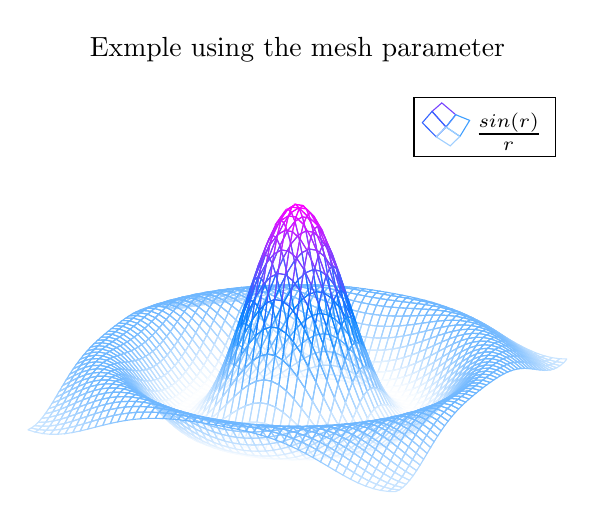
\begin{tikzpicture}
	\begin{axis}
		[
		title=Exmple using the mesh parameter,
		hide axis,
		colormap/cool,
		]
		\addplot3[
			mesh,
			samples=50,
			domain=-8:8,
			]
			{sin(deg(sqrt(x^2+y^2)))/sqrt(x^2+y^2)};
		\addlegendentry{$\frac{sin(r)}{r}$}
\end{axis}
\end{tikzpicture}
\end{document}
